
\section{An improved Metropolis-Hasting algorithm}

Our main idea is to symmetrize the probability of $W$ under the old and new 
$\theta$, so that the term
$p(W|\theta)$ disappears from the acceptance probability. This will result
in a simpler, and significantly more efficient MCMC scheme.
%This forms the main contribution of this paper.

As before, the MCMC iteration begins with the pair $(S(t), \theta)$. 
Instead of simulating the thinned events $U$, we first generate a new parameter 
$\theta^*$ from some distribution $q(\theta^*|\theta)$. Treat this as an 
auxiliary variable, so that the augmented space now is the triple 
$(S(t), \theta,\theta^*)$. We now pretend $S(t)$ was sampled by a 
uniformization scheme where the bounding rate is given by 
$(\Omega(\theta) + \Omega(\theta^*))$ instead of just $\Omega(\theta)$.
We thus sample the set of thinned events $U$ from a piecewise-constant
Poisson process with intenstity $\Omega(\theta) + \Omega(\theta^*) - 
A_{S(t)}$. The result is that $W$, the union of these events with the actual
trajectory transition times $T$, is a realization of homogeneous Poisson
process with rate $\Omega(\theta) + \Omega(\theta^*)$. We now discard all MJP 
state information, so that the MCMC state space consists of $W$, the current
MJP parameter $\theta$, and the auxiliary parameter $\theta^*$.
Finally, we make an MH proposal that swaps $\theta$ with $\theta^*$. 
Observe from
symmetry that the Poisson skeleton $W$ has the same probability both
before and after this proposal, so that unlike the previous scheme,
the ratio $p(W|\theta^*)/p(W|\theta)$ does not appear in the acceptance 
ratio. This simplifies computation, and significantly improves mixing.
The acceptance probability 
%depends only on the probability of the observations
%under both set of parameters, %as we can use the forward-backward algorithm
%to calculate this. Our acceptance probability 
is given by
$$ \text{acc} = 
  \min\left(1, \frac{p(X,\theta^*)q(\theta|\theta^*)}
   {p(X,\theta)q(\theta^*|\theta)}\right) = 
  \min\left(1, \frac{p(X|\theta^*)p(\theta^*)q(\theta|\theta^*)}
   {p(X|\theta)p(\theta)q(\theta^*|\theta)}\right).
   $$
   The terms $p(X|\theta^*)$ and  $p(X|\theta)$ can be calculated by 
   running a forward pass of the forward-backward algorithm. Having
   accepted or rejected the proposal, a new trajectory is sampled by
   completing the backward pass, after which the thinned events are
   discarded. We sketch out our algorithm in 
   figure~\ref{fig:MH_improved} and algorithm~\ref{alg:MH_improved}.
\setlength{\unitlength}{0.8cm}
  \begin{figure}[H]
  \centering
  \begin{minipage}[!hp]{0.45\linewidth}
  \centering
    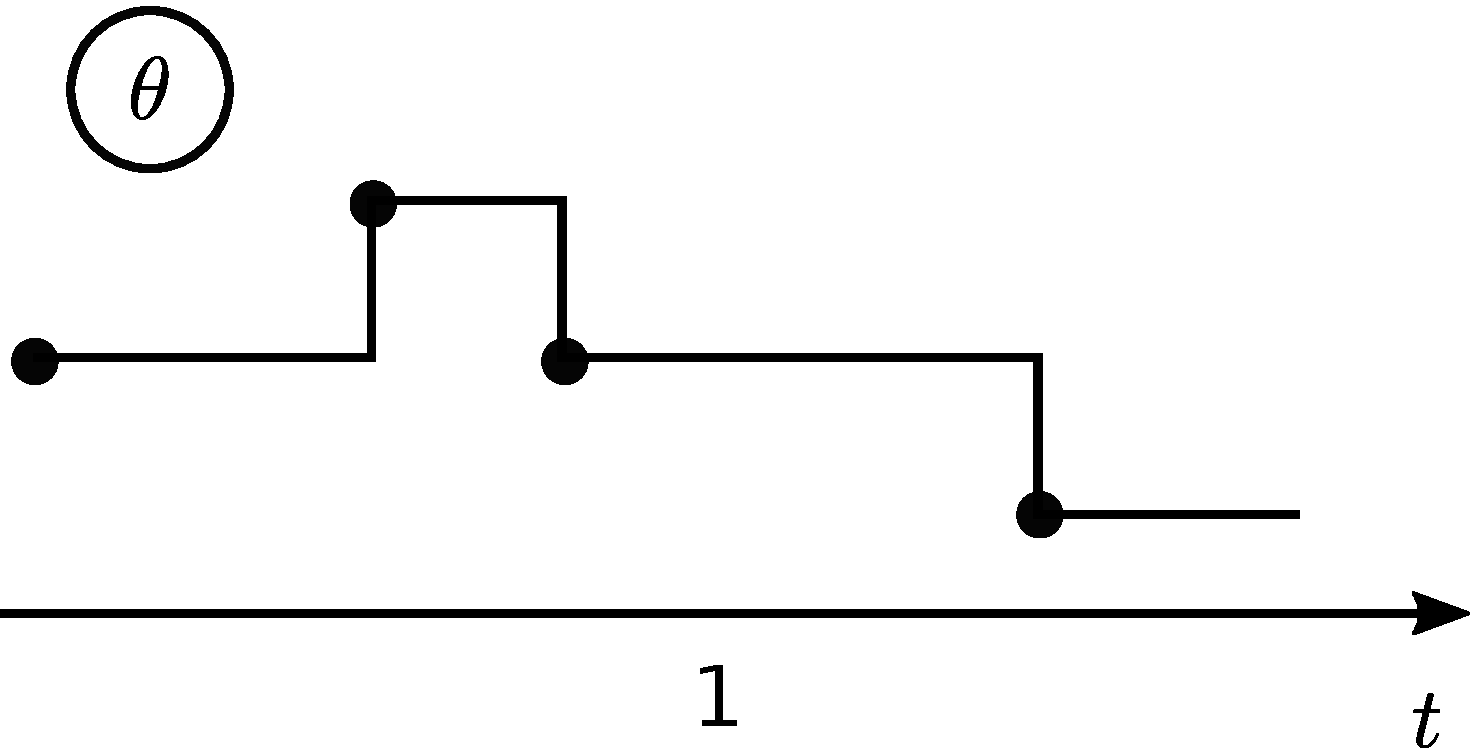
\includegraphics [width=0.70\textwidth, angle=0]{figs/plot0.pdf}
      \end{minipage}
  \begin{minipage}[hp]{0.45\linewidth}
  \centering
    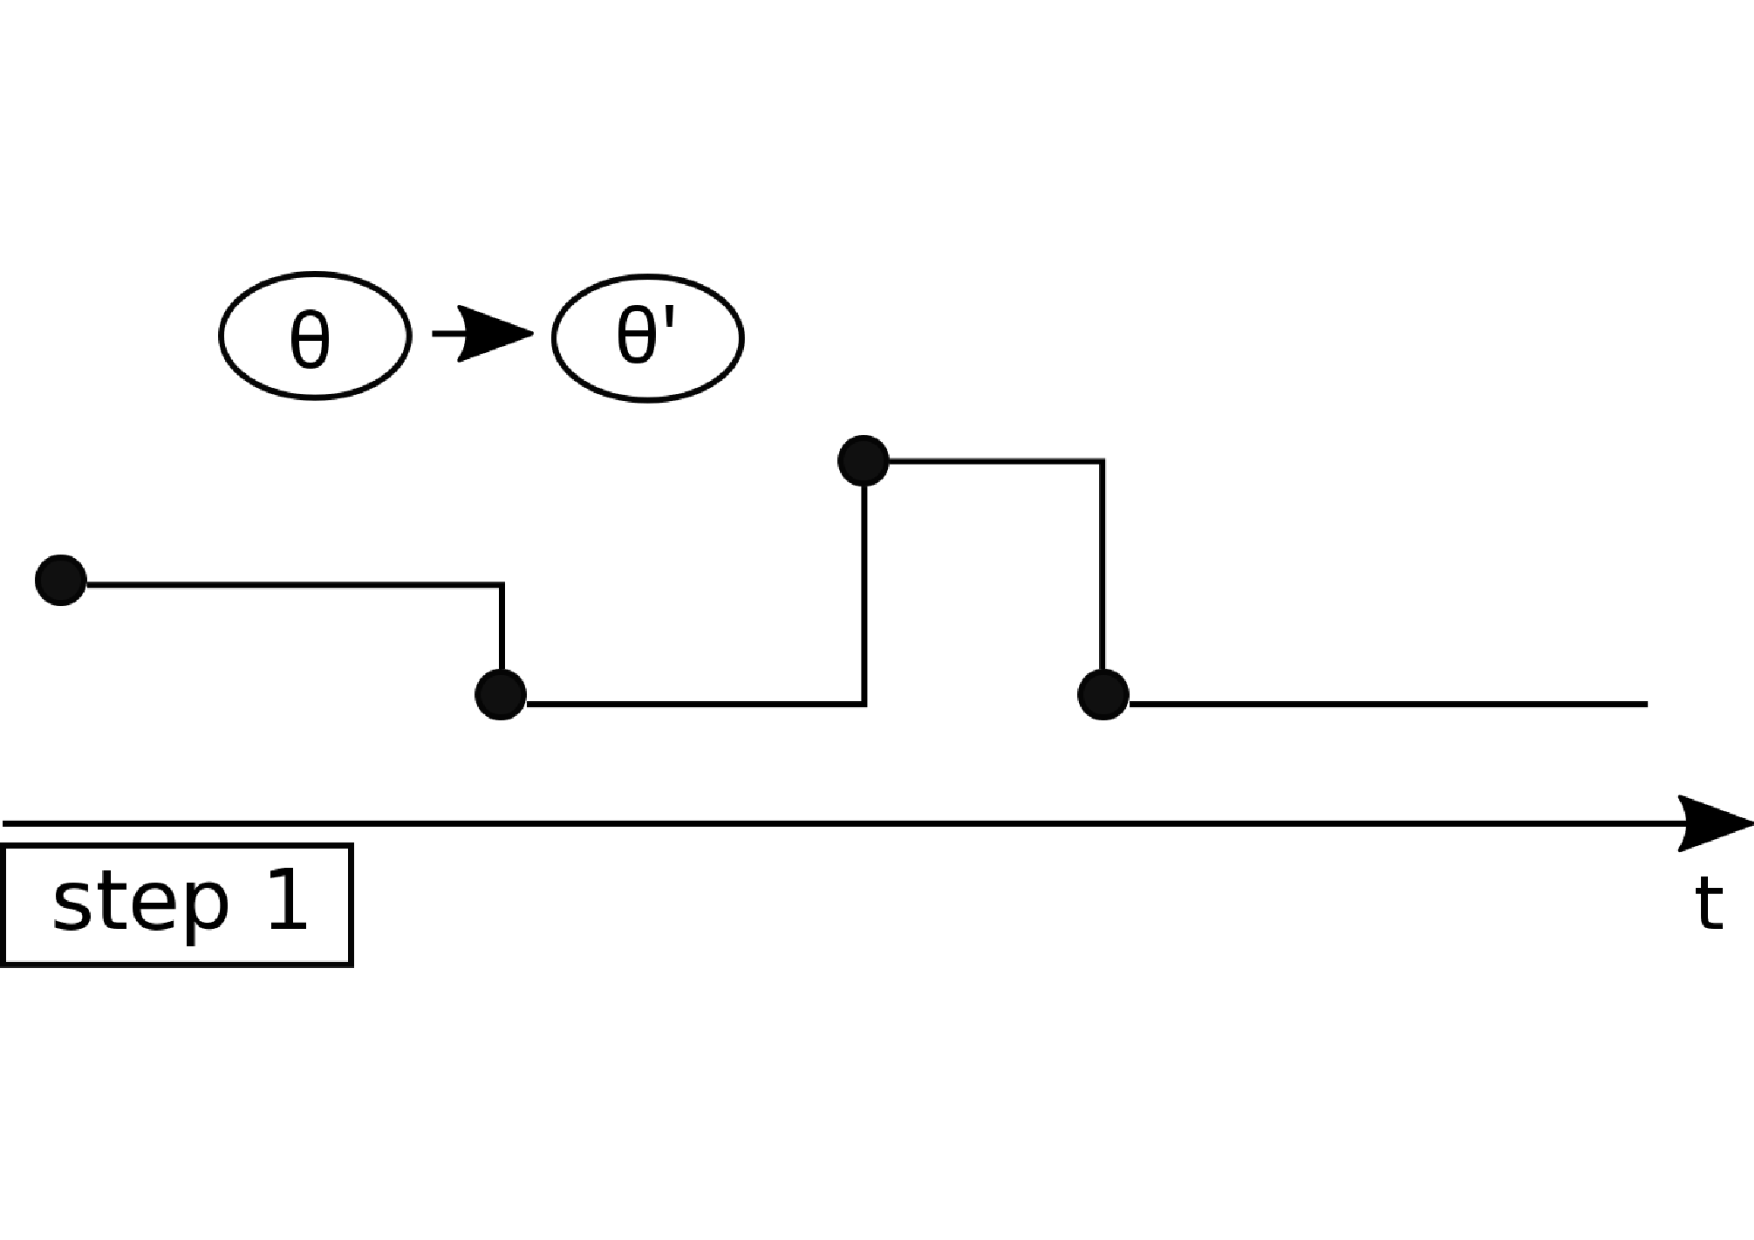
\includegraphics [width=0.70\textwidth, angle=0]{figs/plot1.pdf}
    \vspace{-0 in}
  \end{minipage}
  \begin{minipage}[hp]{0.45\linewidth}
  \centering
    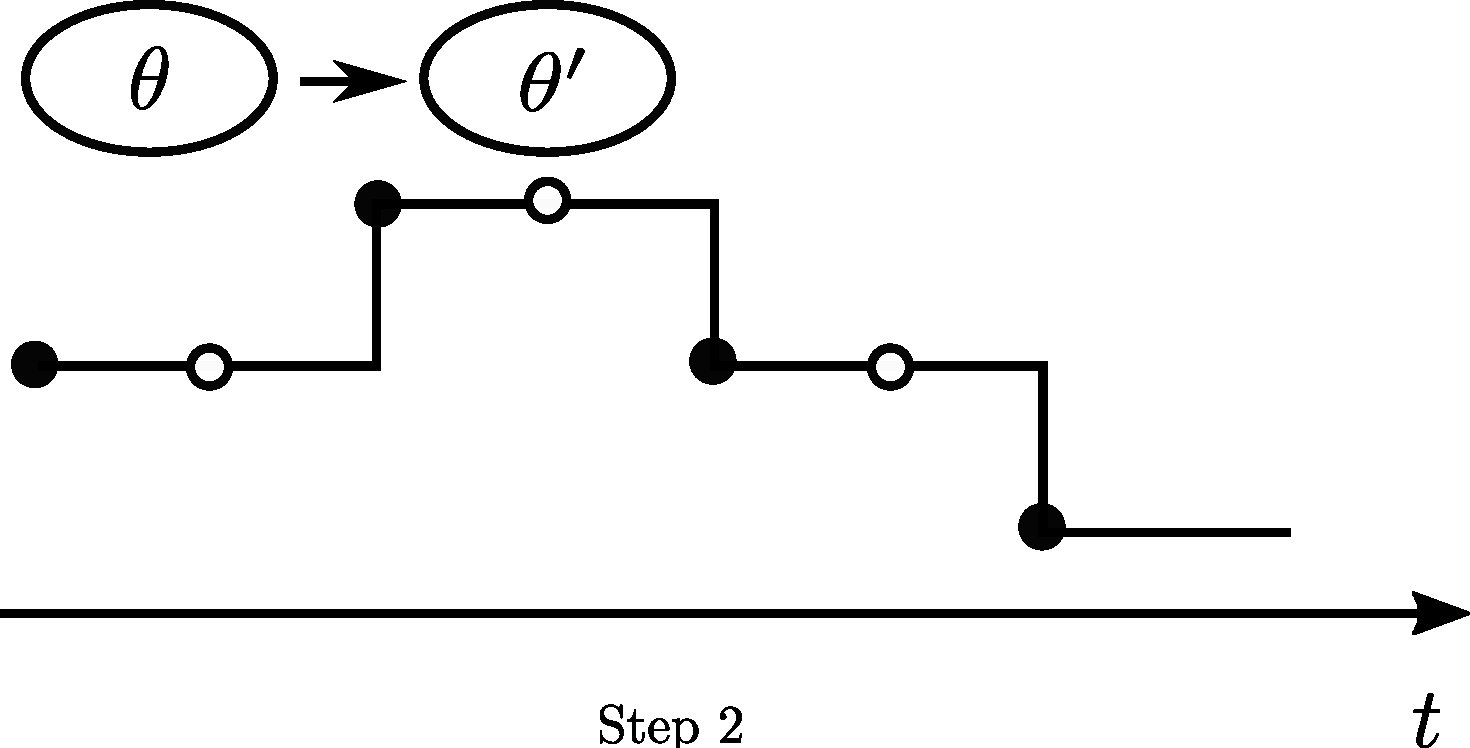
\includegraphics [width=0.70\textwidth, angle=0]{figs/plot2.pdf}
    \vspace{-0 in}
  \end{minipage}
  \begin{minipage}[hp]{0.45\linewidth}
  \centering
    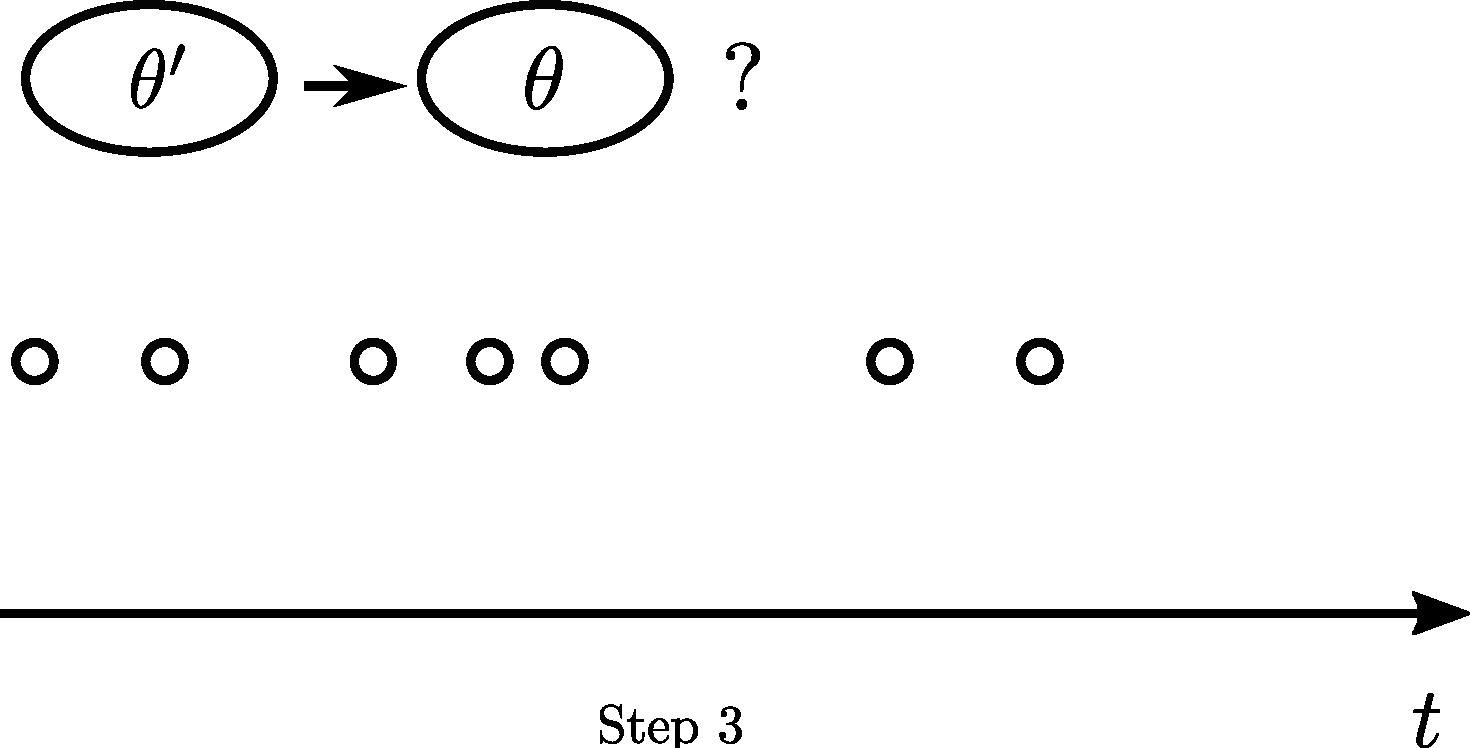
\includegraphics [width=0.70\textwidth, angle=0]{figs/plot3.pdf}
    \vspace{-0 in}
  \end{minipage}
% \begin{minipage}[hp]{0.45\linewidth}
% \centering
%   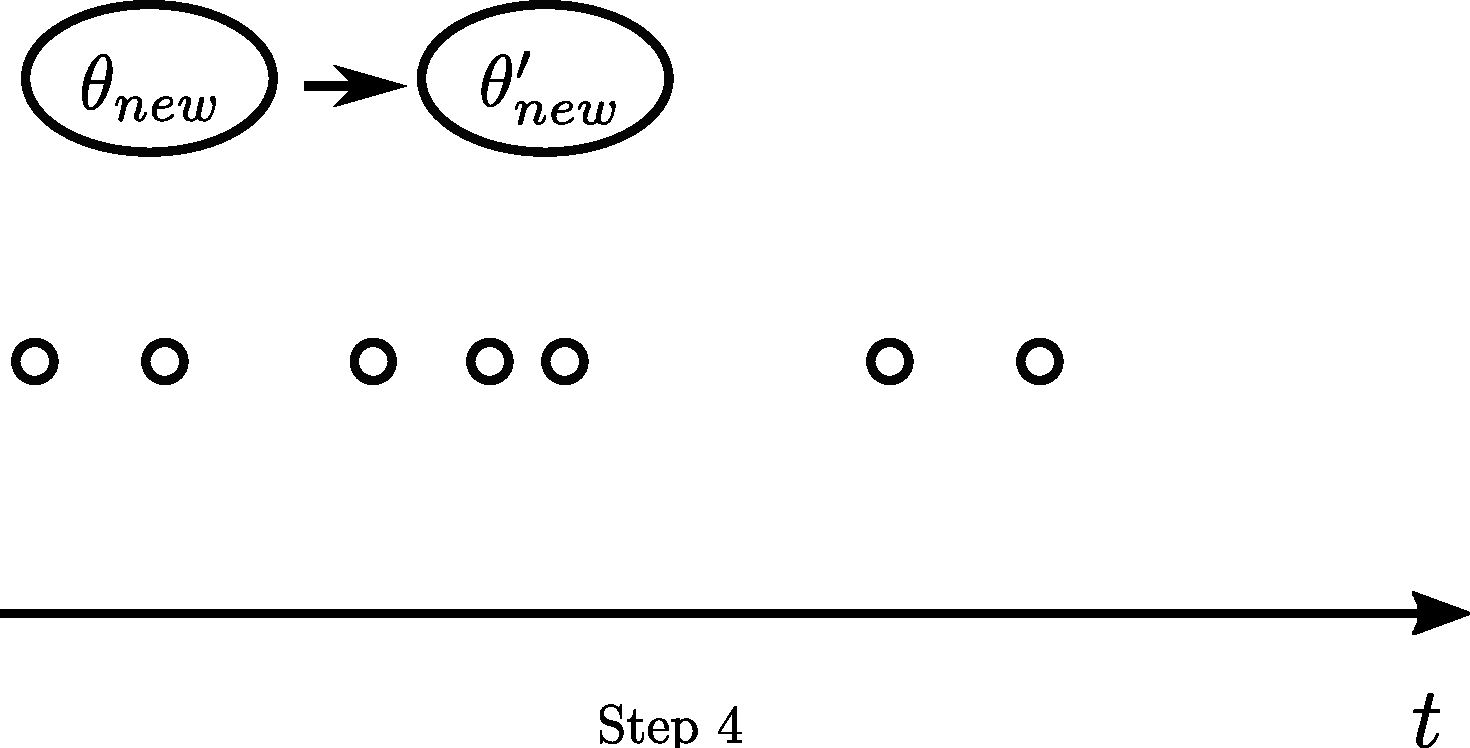
\includegraphics [width=0.70\textwidth, angle=0]{figs/plot4.pdf}
%   \vspace{-0 in}
% \end{minipage}
  \begin{minipage}[hp]{0.45\linewidth}
  \centering
    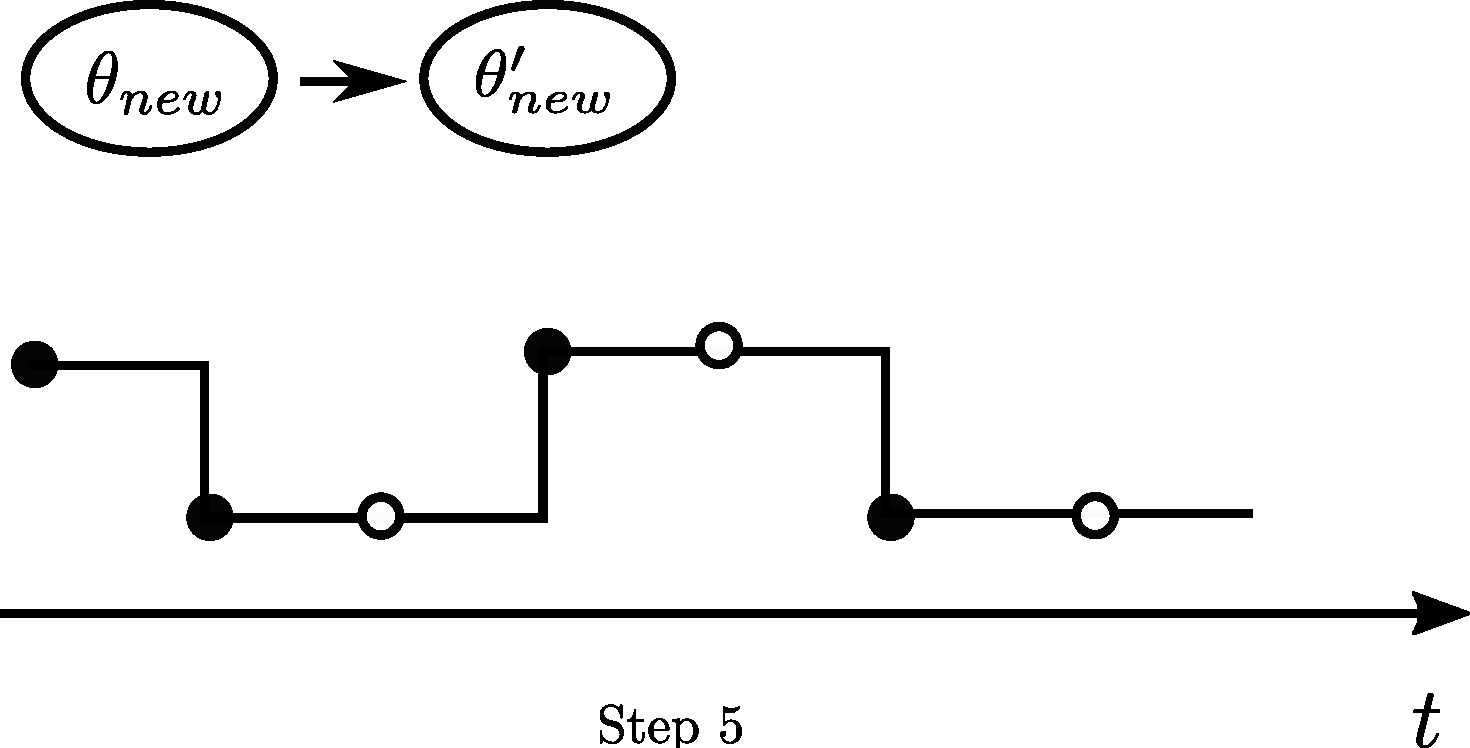
\includegraphics [width=0.70\textwidth, angle=0]{figs/plot5.pdf}
    \vspace{-0 in}
  \end{minipage}
  \begin{minipage}[hp]{0.45\linewidth}
  \centering
    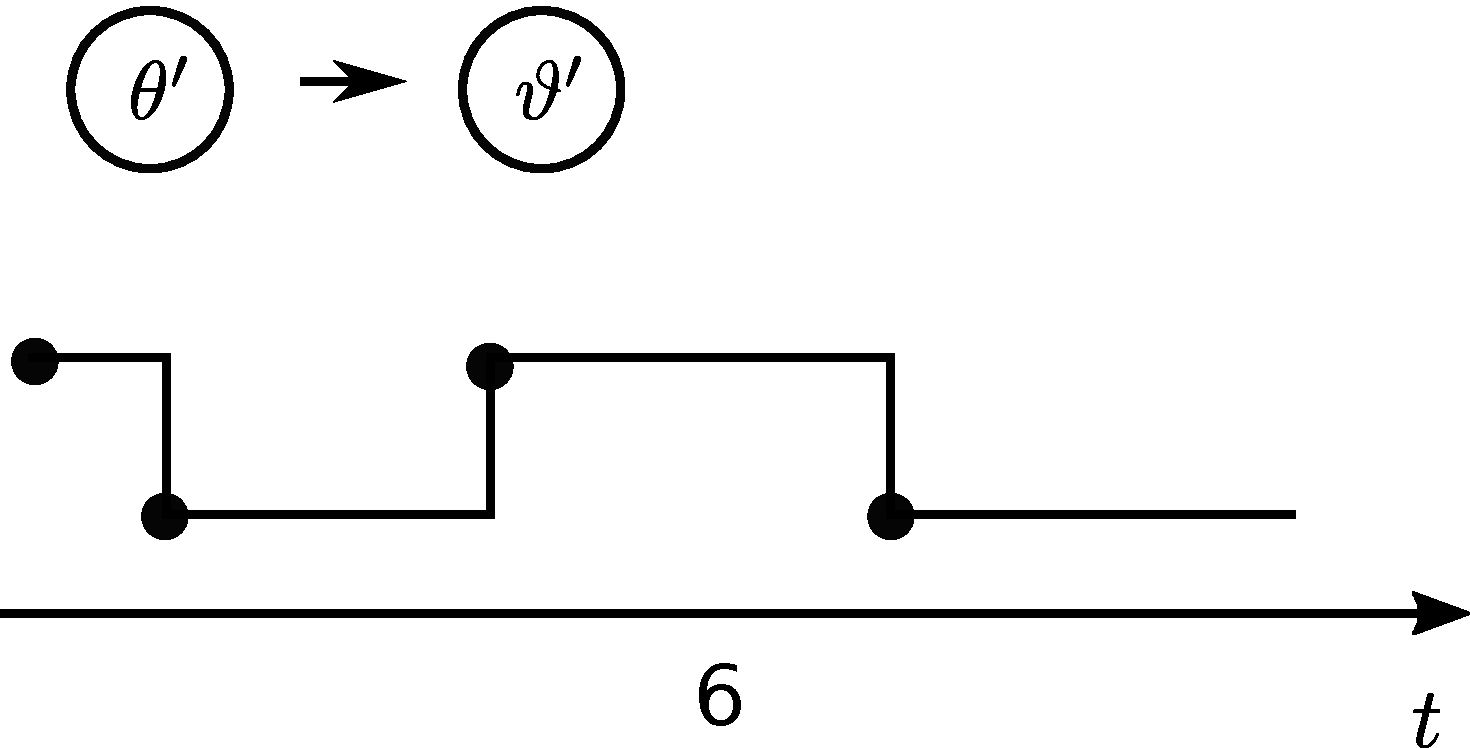
\includegraphics [width=0.70\textwidth, angle=0]{figs/plot6.pdf}
    \vspace{-0 in}
  \end{minipage}
    \caption{Steps 0-3: Starting with a trajectory and parameter $\theta$,
      simulate an auxiliary parameter $\theta'$, and then the thinned events
      $U$ from a rate $\Omega(\theta) + \Omega(\theta') - A_{S(t)}$ Poisson
      process. Step 4: Propose swapping $\theta$ and $\theta'$. Step 5:
      Run a forward pass to accept or reject this proposal, and use the accepted
    parameter to simulate a new trajectory. Step 6: Discard the thinned events.} 
   \label{fig:MH_improved}

  \end{figure}

\begin{algorithm}[H]
   \caption{Improved MH for parameter inference for MJPs }
   \label{alg:MH_improved}
  \begin{tabular}{l l}
   \textbf{Input:  } & \text{A set of partial and noisy observations $X$}, \\
                      & \text{The previous MJP path $S(t) = (S, T)$, the previous MJP parameters $\theta$}.\\ 
                     & \text{A  Metropolis-Hasting proposal $q(\cdot | \theta)$}.\\
   \textbf{Output:  }& \text{A new MJP trajectory $\tilde{S} (t) = (\tilde{S}, \tilde{T})$, 
                            new MJP parameters $\tilde{\theta}$}.\\
   \hline
   \end{tabular}
   \begin{algorithmic}[1]
      \State Sample $\theta^* \sim q(\cdot| \theta)$, and 
      set $\Omega = \max_i A_i(\theta) + \max_i A_i(\theta^*)$. 
      %In the case of uniformization, we
      %have a single $\Omega$ for all states, with $\Omega = \max_i A_i(\theta) + \max_i A_i(\theta^*)$.
      %, with $h(\theta) > max_s{|A_s(\theta)|}$, $h(\theta^*) > max_s{|A_s(\theta^*)|}$ using some deterministic function $h$.
    \State Sample virtual jumps $U\subset[t_{start}, t_{end}]$ from a nonhomogeneous Poisson process with 
    piecewise-constant rate $R(t) = (\Omega - A_{S(t)}(\theta))$. 
    Define $W = T \cup U$ and discard all MJP state information.
    \State The current MCMC state-space is $(W,\theta,\theta^*)$. Propose swapping
    $\theta$ and $\theta^*$, so that the new state-space is 
    $(W, \theta^*, \theta)$. The acceptance probability is given by
   % accept $\theta^*$ as $\tilde{\theta}$ with probability $\alpha$.
        \begin{align*}
        \alpha %&=  1 \wedge \frac{P(W,(\theta^*, \theta)| y)}{P(W, (\theta, \theta^*)| y)}\\
       % &=  1 \wedge \frac{P(y| W,\theta^*, \theta) P(W | (\theta^*, \theta))p((\theta^*, \theta))}{P(y| W,(\theta, \theta^*)) P(W | (\theta, \theta^*))p((\theta, \theta^*))}\\
        &=  1 \wedge \frac{p(X| W,\theta^*)p(\theta^*)q(\theta|\theta^*)}
        {p(X| W,\theta)p(\theta) q(\theta^*|\theta)}.
        \end{align*}
    \State For both $\theta$ and $\theta^*$, make a forward pass through the 
    elements of $W$, sequentially updating the distribution over states at 
    $w \in W$ given observations upto $w$. At the end, we have calculated
    $p(X|W,\theta)$ and $p(X|W,\theta^*)$. Use these to accept or reject the
    proposed swapping of $\theta$ and $\theta^*$. Write the new state space
    as $(W,\tilde{\theta},\tilde{\theta}^*)$.
    \State For the new parameter $\tilde{\theta}$, make a backward pass through 
    the elements of
    $W$, sequentially assigning a state to each element of $W$.
%    Sample a path $\tilde{V}$, from a discret-time Markov chain with $|W| + 1$ steps, using FFBS algorithm. The transition matrix of the Markov chain is $B = (I + \frac{A(\tilde{\theta})}{\Omega})$ while the initial distribution over states is $\pi_0$. The likelihood of state $s$ at step $i$ is 
%    $$ L_i(s) = P(Y_{[w_i, w_{i + 1})} | S(t) = s \; for\; t \in [w_i, w_{i + 1})) = \prod_{j: t_j \in [w_i, w_{i + 1})}p(y_{t_j} | S(t_j) = s).$$\\
%%(i.e. $V(i) \sim P(V |  \theta(i), W(i - 1), y).$) Then delete all the virtual jumps to get $S(i), T(i) .$\\
    \State Let $\tilde{T}$ be the set of times in $W$ when the Markov chain changes state. Define $\tilde{S}$ as the corresponding set of state values. Return $(\tilde{S}, \tilde{T}, \tilde{\theta})$.
\end{algorithmic}
\end{algorithm}

